\begin{frame}
  \frametitle{Motivation}
  \begin{block}{Why model Pyroprocessing?}
  	\begin{itemize}
  		\item No commercial plants.
  		\item Safeguard by design.
  	\end{itemize}
  \end{block}
 \begin{block}{What is the goal?}
 	PyRe will be used to answer the following questions
 	\begin{itemize}
 		\item What is the effect of introducing pyroprocessing plants in the fuel cycle?
 		\item How do various facility designs affect throughput and efficiency?
 		\item Where in a pyroprocessing plant will monitoring most 
 		effectively detect material diversion?
 	\end{itemize}
\end{block}
The first two can be directly answered by the archetype. The third requires data analysis via
diversion algorithms.	
\end{frame}

\begin{frame}
  \frametitle{Diversion}
        \begin{figure}
        	\centering
        	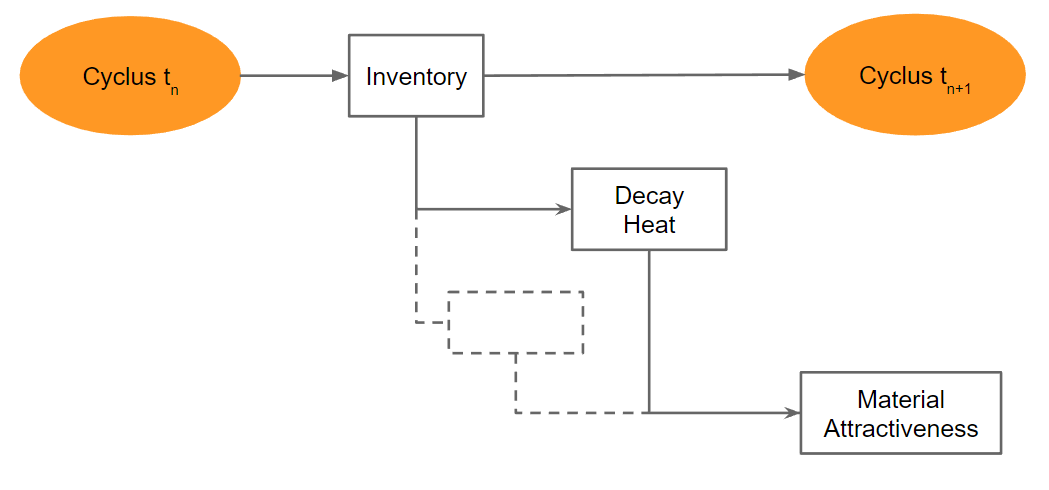
\includegraphics[width=0.9\linewidth]{diversion1}
        	\caption{Diversion detection methods within Cyclus \ref{cyclus-dev}.}
        \end{figure}
\end{frame}
